\section{Sieci neuronowe i algorytmy}

W chwili pisania tej pracy do klasyfikacji i detekcji obiektów na obrazie wykorzystywano kilka różnych sieci neuronowych. Sieci te wykorzystują kilka bazowych algorytmów --- wybór regionów obrazu do analizy jest decydującym czynnikiem dla każdego z algorytmów.
 
\subsection{R---CNN Region---Convolutional Neuron Network}

Sieci typu R-CNN zostały stworzone w celu umożliwienia szybkiej detekcji obiektów, ich lokalizacji i klasyfikacji. Sygnałem wejściowym podawanym wytrenowanej sieci jest obraz. Odpowiedzią sieci R-CNN jest zestaw koordynat ramek (ang: bounding boxes) obejmujących wykryte obiekty oraz nazwa klasy do której je zakwalifikowano. Algorytm ewoluował z sieci CNN kolejno do:
\begin{itemize}
	\item R---CNN
	\item Fast---R---CNN
	\item Faster---R---CNN
\end{itemize}

Głównymi problemami blokującymi możliwość wykorzystania sieci typu R---CNN do detekcji obiektów w czasie rzeczywistym między innymi:
\begin{itemize}
	\item trenowanie sieci jest skomplikowane i zabiera bardzo dużo czasu
	\item trening odbywa się w wielu fazach (np.: trening klasyfikacji versus nauka wyboru odpowiednich regionów do obróbki)
	\item sieć jest bardzo wolna na etapie wnioskowania (szczególnie kiedy ma do czynienia z danymi, które nie były objęte szkoleniem)
\end{itemize}

\subsection{SSD --- Single Shot MultiBox Detector}
Algorytm opracowany przez C. Szegedyat al.\cite{DBLP:journals/corr/LiuAESR15} na przełomie roku 2016/2017. Dedykowany do szybkiej detekcji obiektów w obrazie wideo. Nazwa algorytmu wzięła się od z opisu jego działania:
\begin{itemize}
	\item Single Shot - lokalizacja obiektu i jego klasyfikacja wykonywana jest w jednym przebiegu sieci
	\item MultiBox - nazwa techniki opracowanej przez Szegedy'ego et al. 
	\item Detector - sieć jest detektorem obiektów i wykonuje ich klasyfikacji
\end{itemize}

Sieci SSD budowane są w architekturze opartej na modelu VGG-16, bez warstw fully connected. Głównym powodem użycia VGG-16 jako sieci wyjściowej była wydajność tego modelu i jak również popularność (dostępność wielu modeli gotowych do transfer learning). 
W budowie sieci zamiast warstw fully connected zastosowano zestaw konwulcyjnych warstw pomocniczych --- właściwa detekcja odbywa się w większej skali progresywnie zmniejsza rozmiar wejść do każdej następnej warstwy.
\begin{figure}[ht]
	\centering
	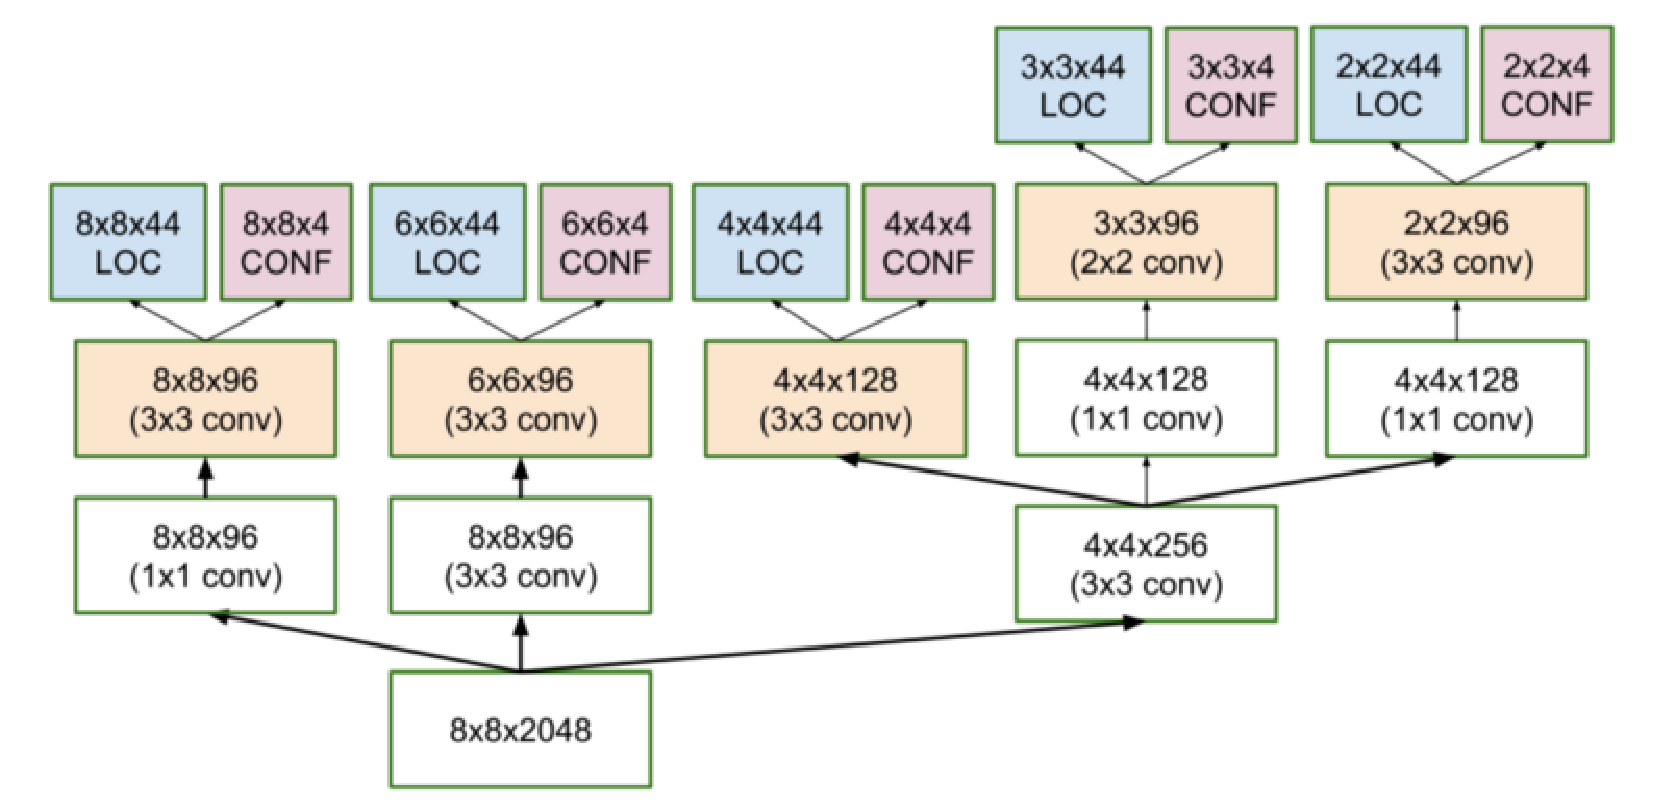
\includegraphics[width=\textwidth]{fig/ssd.pdf}
	\caption{Budowa wielkoskalowego konwulsyjnego przewidywania lokalizacji multiboksów. źródło: \cite{DBLP:journals/corr/LiuAESR15}}
	\label{fig:ssd}
\end{figure}

Technika  MultiBox wytycza szybko koordynaty ramek (bounding boxes) otaczających obiekty bez wiedzy o ich klasie. Rys \ref{fig:ssd} pokazuje w jaki sposób redukowany jest liczba wymiarów ramek.


\subsection{Framework'i}
Algorytmy implementowane są w różnych wariantach i dostępne jako gotowe biblioteki w kilku framework\'ach.\todo{uzupełnić: Theano, Keras, Tensorflow, Detectron}

\subsection{Architektura sieci}

\subsubsection{AlexNet}
Historycznie biorąc AlexNet jest pierwszą z sieci neuronowych wykorzystywanych do detekcji obiektów w obrazie wideo, która była znacząco podnieść poziom dokładności wykrywania w rankingu ImageNet Classification. Składa się ona z 5 konwulcyjnych warstw i następujących po nich trzech w pełni połączonych warstw. Struktura zaproponowana przez Alex\'a Krizhevsky\'ego wyróżniała się również zastosowaniem funkcji aktywacji ReLu (Rectified Linear Unit) zamiast tradycyjnie stosowanych funkcji tangens hiperboliczny czy sigmo-idów.
ReLu definiowana jest jako:
\begin{equation} \label{eq:relu}
f(x)=max(0,x)
\end{equation}
Dużą przewagą funkcji \ref{eq:relu} nad poprzednio powszechnie używanymi funkcjami (tanh i sigmoid) jest szybkość uczenia się. Dzieje się tak dlatego, że po przekroczeniu pewnej wartości zarówno funkcja tanh jak i sigmoid wchodzi w stan nasycenia i zmiany impulsu wejściowego nie powodują, bądź powodują bardzo małe zmiany na wyjściu --- stan ten jest nazywany problemem zanikającego gradientu (ang.: vanishing gradient problem)
\begin{figure}[htp]	
	\centering
	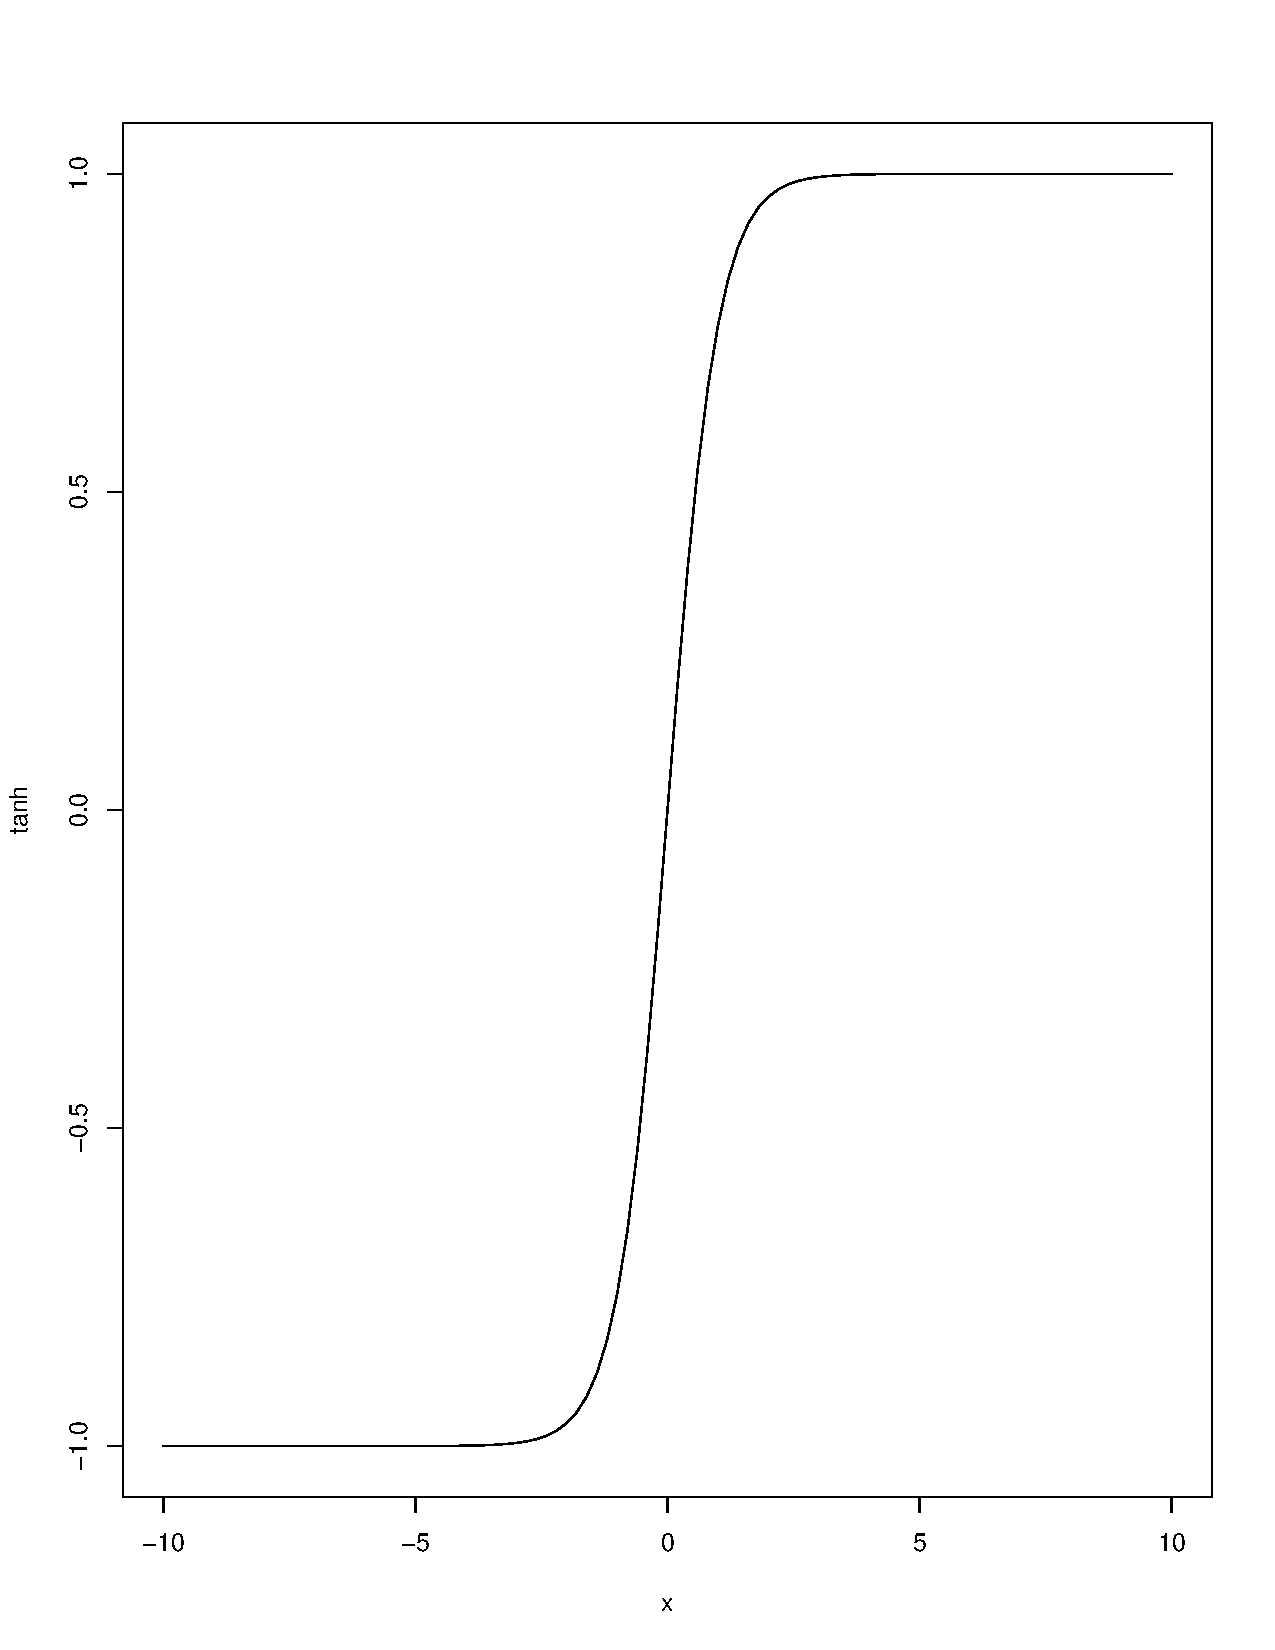
\includegraphics[width=.3\textwidth]{fig/tan.pdf}\hfill
	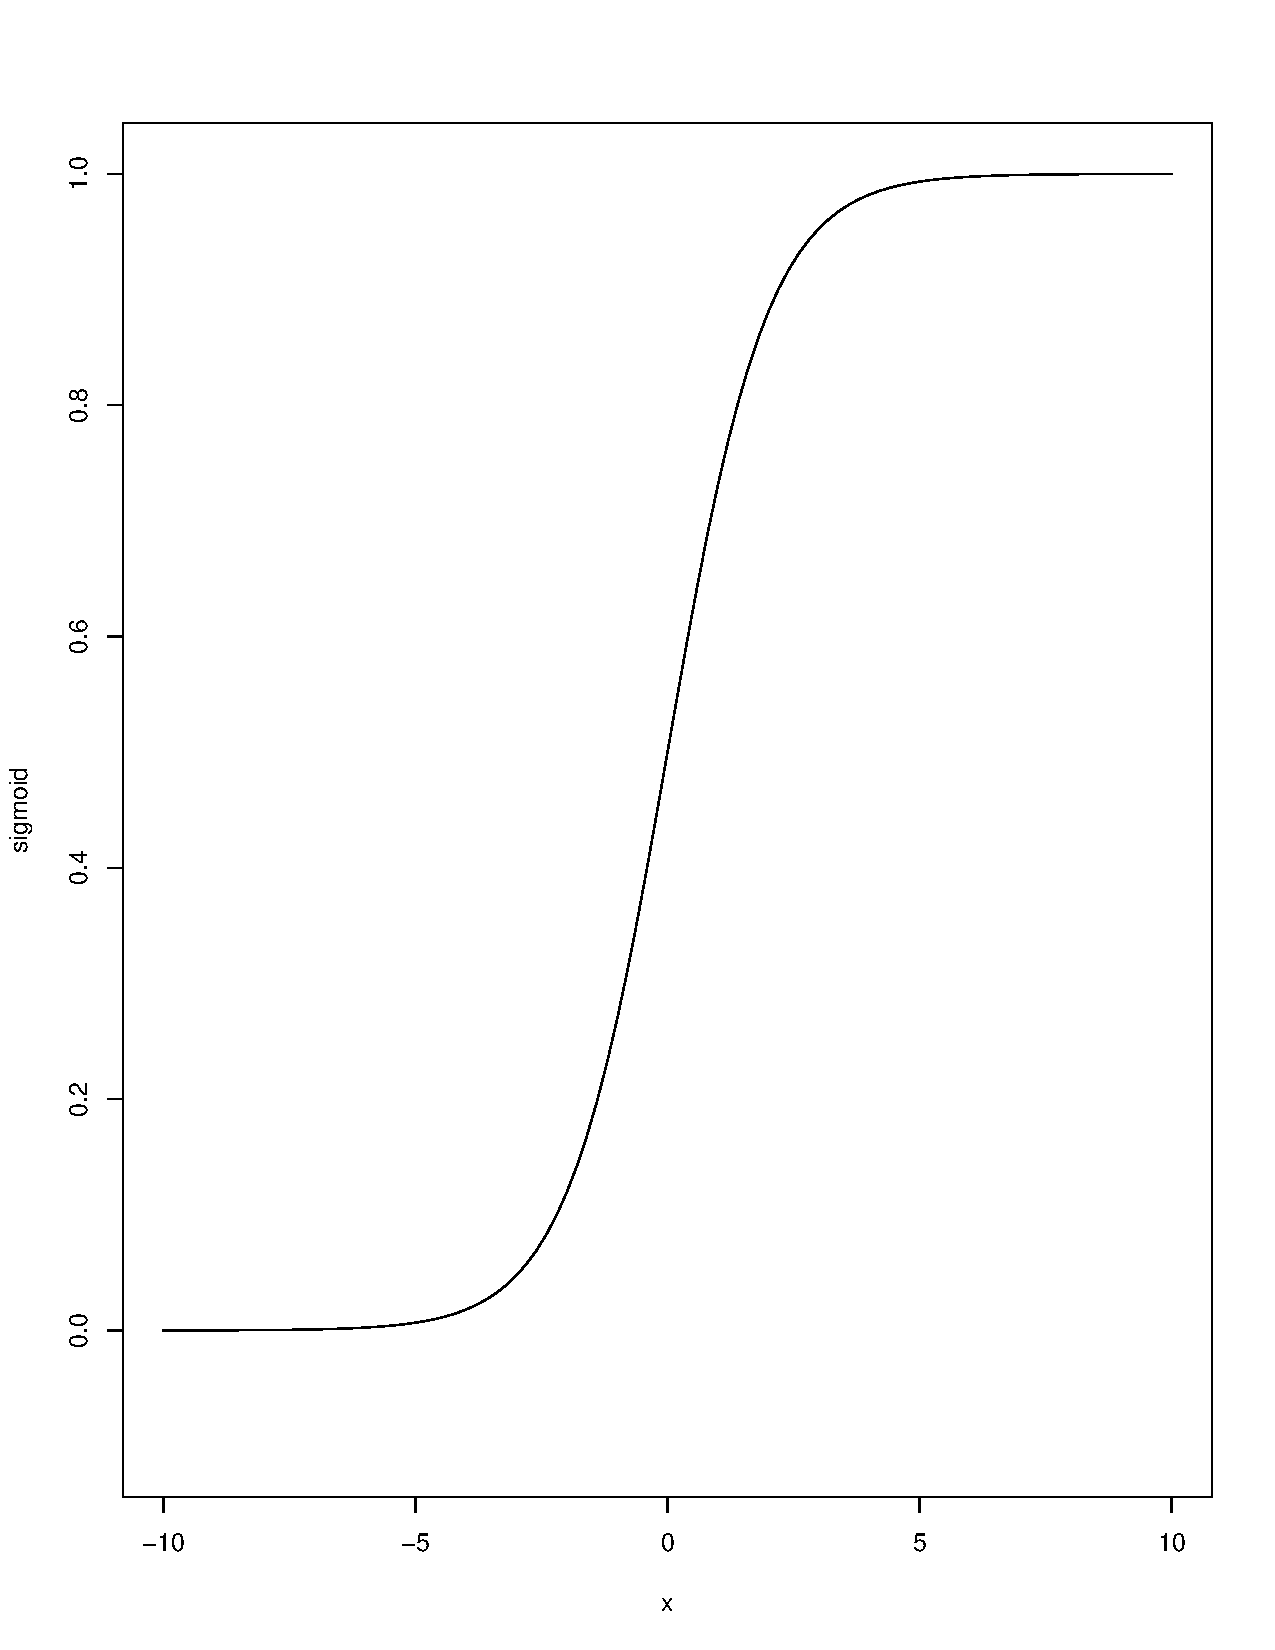
\includegraphics[width=.3\textwidth]{fig/sigm.pdf}\hfill
	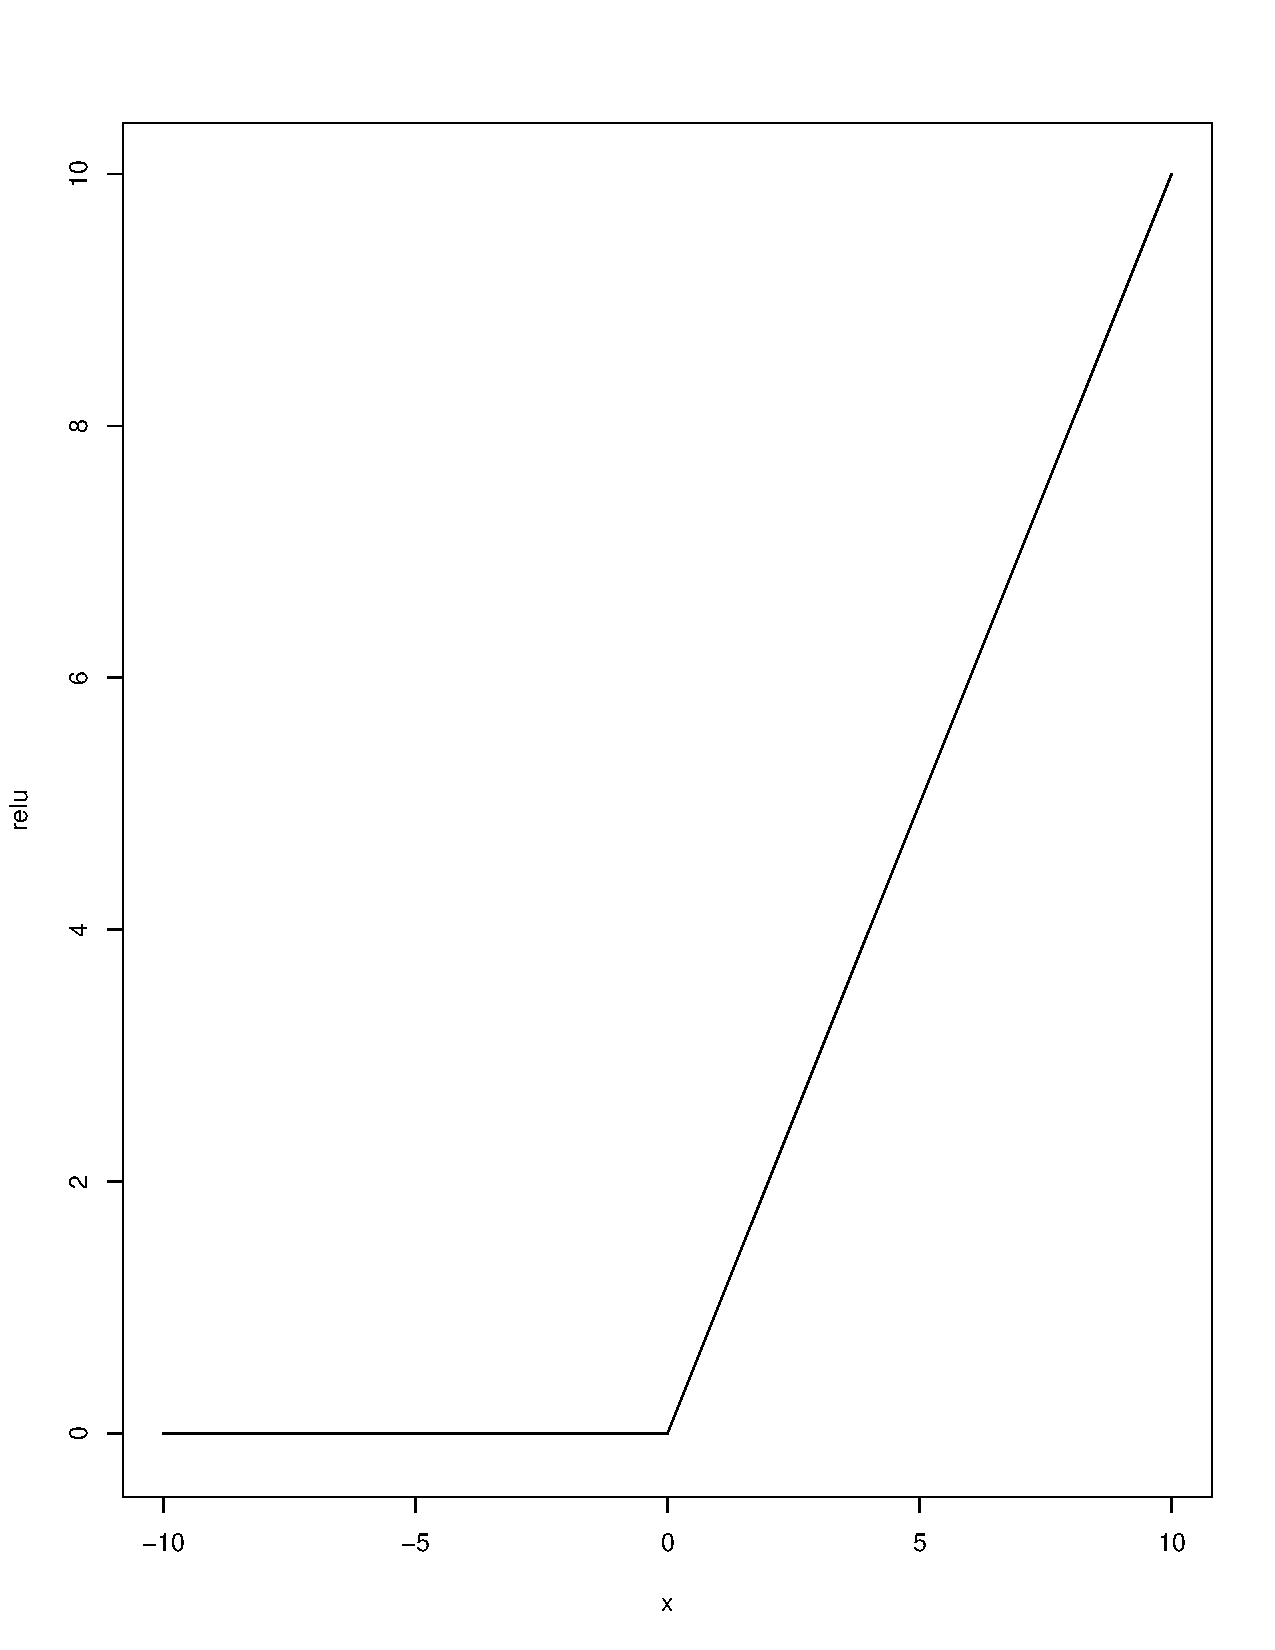
\includegraphics[width=.3\textwidth]{fig/relu.pdf}	
	\caption{Funkcje aktywujące: kolejno tangens hiperboliczny, sigmoid, ReLu}
	\label{fig:relu}	
\end{figure}
Dodatkowo, aby ograniczyć przetrenowanie sieci po każdej warstwie w pełni połączonej dodano warstwę Dropout --- każdy neuron z określonym prawdopodobieństwem $p$ może zostać wyłączony. 

\subsubsection{VGG---16}
Grupa VGG z Oxfordu udoskonaliła AlexNet poprzez usunięcie dużych filtrów i zastąpiła je wieloma filtrami mniejszymi. Z jednej strony zmiejszyło to potrzebny nakład mocy obliczeniowej, z drugiej zwiększył głębokość sieci --- co za tym idzie zdolność do nauki bardziej skomplikowanych schematów.

\subsubsection{GoogLeNet/Inception}\cite{43022}
Ponieważ VGG---16 cechowała niezwykła dokładność przy bardzo dużym nakładzie mocy obliczeniowej i pamięci potrzebnej do zaimplementowania sieci, Google rozpoczęło prace nad udoskonaleniem modelu VGG. Rezultatem tego jest właśnie GoogLeNet --- cechą charakterystyczną jest warstwa wejściowa (Inception)\cite{ai_gitbook}. Warstwa Inception aproksymuje rzadką sieć CNN z sieci o normalnej gęstości. Z właściwości złożonych sieci neuronowych wynika, że tylko niewielka ilość neuronów jest skuteczna -- ilość filtrów jest również redukowana. Do wychwycenia detali aplikowane są filtry o różnych wielkościach i o różnej skali. 
\begin{figure}[htp]	
	\centering
	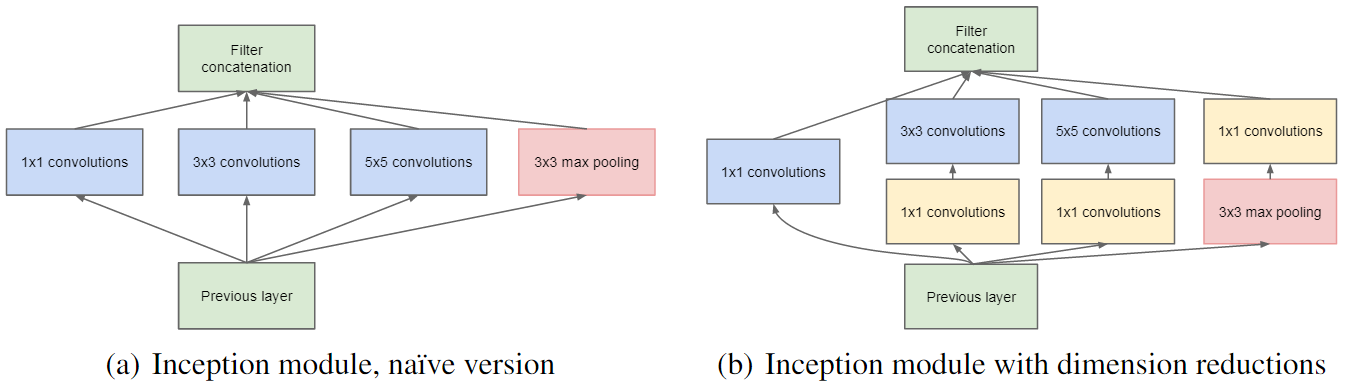
\includegraphics[width=.3\textwidth]{fig/inception_1x1.png}\hfill
	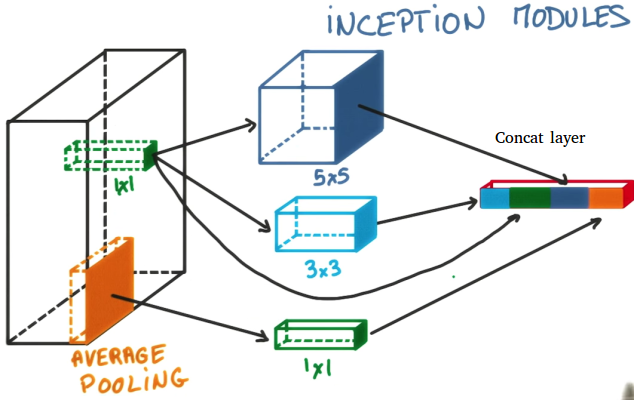
\includegraphics[width=.3\textwidth]{fig/InceptionModules.png}\hfill
	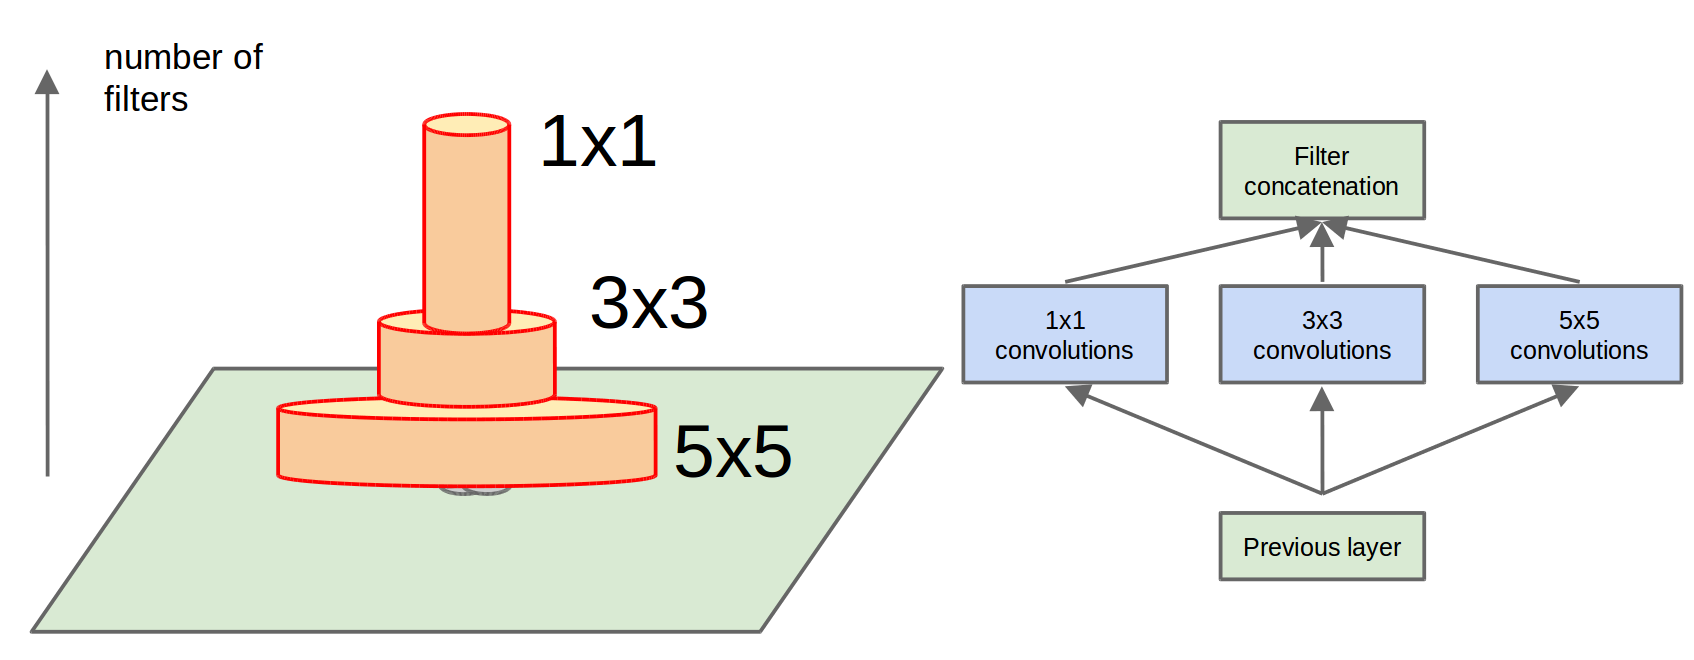
\includegraphics[width=.3\textwidth]{fig/Naive_VersionNception.png}	
	\caption{GoogLeNet}
	\label{fig:GoogLeNet}	
\end{figure}


\subsubsection{Residual Networks}
Zwiększanie głębokości sieci neuronowej (ilości warstw ukrytych) prowadzi do zwiększenia dokładności sieci jeśli zwracamy dużą uwagę na przetrenowanie sieci i do niej nie doprowadzimy. Im większa głębokość sieci, tym sygnał potrzebny do zmiany wag jest mniejszy. Maleje on wraz z ilością warstw. Łatwo zauważyć, że pierwsze warstwy tracą na ważności -- zjawisko to nazywa się zanikającym gradientem. Oczywiście optymalizacja głębokiej sieci jest też dużo bardziej skomplikowana ze względu na ilość współczynników wag do dostrojenia.Problemy te częściowo rozwiązują sieci rezydualne.
Sieci rezydualne usprawniają szkolenie głębokich sieci poprzez zastosowanie modułów zwanych modułami rezydualnymi.
\begin{figure}[ht]
	\centering
	\includegraphics[width=\textwidth]{fig/res1.png}
	\caption{Zasada nauki sieci głębokich przy użyciu modułów rezydualnych}
	\label{fig:residual1}
\end{figure}

\subsubsection{}
next sub
\subsection{Wykrywanie vs klasyfikacja}

\subsubsection{Wykrywanie}
Wykrywanie obiektów wykorzystuje algorytmy klasyfikujące do określenia co i gdzie znajduje się na badanych obrazie (również wideo). Powstanie i rozwój sieci CNN umożliwiło wyrywanie wielu klas przy pojedynczej analizie. Algorytm wykrywający (ang. object detection) po zbadaniu obrazu przedstawi rozmieszczenie na obrazie rozpoznanych obiektów.

\subsubsection{Klasyfikacja}
Klasyfikacja polega na określeniu czy obraz należy do pewnej, z góry określonej kategorii. Np. klasyfikator odpowiada na pytanie --- czy na badanym obrazie znajduje się kot.